\documentclass{standalone}

\usepackage{circuitikz}

\begin{document}

% INT_AY22_L23_Fig01_Grav_system.png

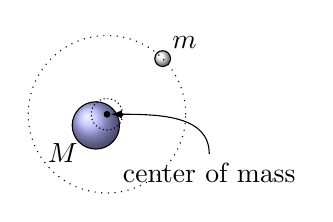
\begin{tikzpicture}[> = latex]

	% Primary w/orbit
	
	\draw [ball color = blue!30] (225 : 0.2) circle (0.3 cm) node [below left = 0.3 em] {$M$};
	\draw [densely dotted] (0, 0) circle (0.2 cm);
	
	% Center of mass
	
	\filldraw (0, 0) circle (1 pt);
	\node (CM-label) at (330 : 1.5) {center of mass};
	\draw [->] (CM-label.north) to [out = 90, in = 0] (0.05, 0);
	
	% Secondary w/orbit
	
	\draw [ball color = gray!10] (45 : 1) circle (0.1 cm) node [above right] {$m$};
	\draw [dotted] (0, 0) circle (1 cm);
	
\end{tikzpicture}

\end{document}